%!TEX root = ../documentation.tex
\chapter{Webpage Fetching}
\label{chap:webpage_fetching}

Recording webpage traces is a critical part of our website fingerprinting approach since all measurements and calculations depend on this data. In this chapter, we present our automated website fetching process used to gather traces. First, we introduce the structure of our fetching tool. Then, we describe its operation and show a small example.

\section{Folder Organization}
\label{sec:fetching_folder}

\begin{listing}[t]
\begin{lstlisting}[basicstyle=\scriptsize\ttfamily,numbers=none]
Timestamp Source-IP:Source-Port > Destination-IP:Destination-Port Packet-Length
\end{lstlisting}
\caption{Extracted raw \ac{TCP} data (based on \cite{Pennekamp2014})}
\label{lst:tcprawdata}
\end{listing}

\begin{listing}[t]
\begin{lstlisting}[basicstyle=\scriptsize\ttfamily,numbers=none]
TimestampStart TimestampEnd OffSet Source-IP Source-Port Destination-IP
Destination-Port Packet-Length
\end{lstlisting}
\caption{Extracted raw \ac{TLS} data}
\label{lst:tlsrawdata}
\end{listing}

Our webpage fetching algorithm is located in the folder \texttt{crawling/}. Figure \ref{fig:crawlingOrdering} shows its organization. Folder \texttt{crawling/} consists of:

\todo[inline]{Fix the size of Figure~\ref{fig:crawlingOrdering} to scale correctly on the whole page!}

\begin{figure}
\footnotesize{\dirtree{%
.1 \HandRight \, crawling.
.2 \HandRight \, dumps.
.3 $\star$ <runidentifier>-<hostname>-<urllist>.raw.
.2 \HandRight \, ips.
.3 $\star$ <runidentifier>-<hostname>-<urllist>.ownips.
.3 $\star$ <runidentifier>-<hostname>-<urllist>.torips.
.2 \HandRight \, log.
.3 $\star$ calculatelog-<runidentifier>-<hostname>-<urllist>.log.
.3 $\star$ duplicates-<runidentifier>-<hostname>-<urllist>.log.
.3 $\star$ fetchlog-<runidentifier>-<hostname>-<urllist>.log.
.3 $\star$ tbb-<runidentifier>-<hostname>-<urllist>.log.
.2 \HandRight \, screenshots.
.3 $\star$ <webpage\_url>.png.
.2 \HandRight \, scripts.
.3 $\star$ check-hs-state.py.
.3 $\star$ launch-browser.py.
.3 $\star$ parse-<format>.py.
.3 $\star$ raw-to-tcp.py.
.3 $\star$ raw-to-tls.py.
.3 $\star$ extract-main.py.
.3 $\star$ ip2cell\_wang\_sanitized.py.
.2 \HandRight \, timestamps.
.3 $\star$ <runidentifier>-<hostname>-<urllist>.log.
.2 \HandRight \, txtdumps.
.3 $\star$ <webpage\_url>.txt.
.2 \HandRight \, <output>.
.3 $\star$ <webpage\_url>.
.2 \HandRight \, tmp.
.3 $\star$ kill-streams.
.3 $\star$ last\_closed\_streams.
.3 $\star$ number-streams.
.3 $\star$ .lock-<hostname>.
.2 \HandRight \, urlLists.
.3 $\star$ <linklist>.
.2 $\star$ ERRORS.txt.
.2 $\star$ clear-all.sh.
.2 $\star$ fetch-and-calculate.sh.
.2 $\star$ kill-all.sh.
.2 $\star$ run-client-torbrowser.sh.
}}
\caption{Structure of folder \texttt{crawling/}}
\label{fig:crawlingOrdering}
\end{figure}

\begin{description}
\item[fetch-and-calculate.sh] The main script executing the collection of webpage traces.
\begin{verbatim}
usage: ./fetch-and-calculate.sh [runidentifier] 
     [timeout] [urlfile]

     Program for recording webpage traces where:

[runidentifier]      A name for an identification of a record.
[timeout]            The program waits for a given timeout in 
                     seconds a webpage to be loaded.
[urlfile]            A text file containing URLs of webpages.
\end{verbatim}
The character \texttt{\_} is a keyword and it should not be used in the parameters. By default, the main script launches the \ac{TBB} and starts loading 10 webpages consequently.

\todo[inline]{Check again the exact number of pages loaded consequently!}

\todo[inline]{Check if the script works correctly when the following option in \texttt{WFP\_config} is enabled:}
\vspace{-4mm}
\begin{verbatim}
conf_FORMATS="Wang-cell"
\end{verbatim}

If \texttt{[runidentifier]} starts with \texttt{wsc}, the main script will load only 1 webpage pro browser starting. Additionally, \texttt{[runidentifier]} should end with \texttt{-FG} or \texttt{-BG} in order to indicate for the rest of the scripts if we process foreground or background data. 

\todo[inline]{As far I remember, this is still not mandatory because the complete automation of the toolbox is still in progress.}

The \texttt{[timeout]} should always be at least 180 (based on our previous experiments). This timeout avoids unnecessary waiting time, while fetching most pages successfully. 
\todo[inline]{We should add how the timeout is used.}
\item[clear-all.sh] A script that cleans old data from all directories used for webpage fetching. Use with caution! This might remove valuable data if the path are not set properly or the data has not been backed up correctly.
\begin{verbatim}
usage: ./clear-all.sh

   Clean all directories used for webpage fetching.
\end{verbatim}
\item[kill-all.sh] A script used to kill all (old) fetching related or disturbing processes. New applications can be added if you think that something is missing.
\item[run-client-torbrowser.sh] A script used to start \ac{TBB} with a certain \ac{URL} list and record the network traces with \texttt{tcpdump}.
\begin{verbatim}
usage: ./run-client-torbrowser.sh [runidentifier]
     [timeout] [urlfile]

     Program for starting a Tor browser with a
     given URL where:

[runidentifier]      A name for an identification of a record.
[timeout]            The program waits for a given timeout in 
                     seconds a webpage to be loaded.
[urlfile]            A text file containing URLs of webpages.
\end{verbatim}

For possible issues with \ac{TBB}, we refer the reader to Appendix~\ref{subsec:tbb_start}.

\item[dumps/] A folder where raw dump files, generated by \texttt{tcpdump}, are saved. The folder is automatically created if it does not exist. \todo[inline]{Add where the temporary TLS data is extracted to!}
\item[ips/] A folder where files containing our own \ac{IP} address (with extension \texttt{ownips}) and the corresponding Tor \ac{IP} addresses (with extension \texttt{torips}) are saved. The folder is automatically created if it does not exist.
\item[log/] A folder where log files are saved.\\ \texttt{fetchlog-<runidentifier>-<hostname>-<urlfile>.log} contains logs from our tools, and \texttt{tbb-<runidentifier>-<hostname>-<urlfile>.log} contains logs from \ac{TBB}. Additionally, the folder might contain the file\\ \texttt{duplicates-<runidentifier>-<hostname>-<urlfile>.log} which includes duplicate webpages that have been removed from the original \ac{URL} list. The folder is automatically created if it does not exist.
\item[screenshots/] A folder in which screenshots of already fetched webpages are stored. This folder is automatically created if it does not exist. Screenshots can later be manually used to check if a page load really was finished successful, or if parts of the page, such as advertisements or images, did not load correctly. Complete page-load errors can already be identified from the textdumps. Screenshots should only be used to look into special page loads.
\item[scripts/] A folder containing all relevant scripts used for webpage fetching:
\begin{description}
\item[launch-browser.py] \textcolor{red}{TODO: Add description!}
\item[raw-to-tcp.py] Extracts \ac{TCP} information from the network traces already captured by \texttt{tcpdump}. The script outputs the fetched data in the form shown in Listing \ref{lst:tcprawdata}. Additionally, the user may choose to extract \ac{TCP} information according to Wang's approach~\cite{Wang2014}. To do this, the option \emph{tcp-Wang-format} needs to be enabled (by default, it is not).
\item[parse-tcp.py] Excludes all traffic from the extracted \ac{TCP} data that is not related to the loading a certain webpage. Then, it builds instances from the \ac{TCP} data, relevant to that webpage, in the form shown in Listing \ref{lst:tcpextracteddata}. The \ac{TCP} instances are saved in separate files for each webpage in a folder \texttt{output-tcp/}. Additionally, the user may choose to converts the \ac{TCP} data extracted for Wang's approach into the text version. This is necessary for the next processing steps in order to generate Wang's features. To do this, the option \emph{tcp-Wang-format} needs to be enabled (by default, it is not).
\item[raw-to-tls.py] Extracts \ac{TLS} information from the network traces already captured by \texttt{tcpdump}. The script outputs the fetched data in the form shown in Listing \ref{lst:tlsrawdata}.
\item[parse-tls.py] Excludes all traffic from the extracted \ac{TLS} records that is not related to the loading a certain webpage. Then, it builds instances from the \ac{TLS} information, relevant to that webpage, with reording the records (see Section \ref{sec:fetching_operation} for details). The output of the script is shown in Listing \ref{lst:tlsextracteddata}. The \ac{TLS} instances are saved in separate files for each webpage in a folder \texttt{output-tls/} and \texttt{output-tls-legacy/} if \emph{legacy} option is enabled. The legacy version does not reorder the \ac{TLS} records (see Section \ref{sec:fetching_operation} for details).
\item[parse-cells.py] Extracts information from the \ac{TLS} instances to recreate Tor cell information, relevant to that webpage. The output of the script is similar to the one shown in Listing \ref{lst:tlsextracteddata}. The cell instances are saved in separate files for each webpage in a folder \texttt{output-cell(-*)/}. Legacy versions use the unordered \ac{TLS} records as input (see Section \ref{sec:fetching_operation} for details). Nosendme versions do not extract Tor sendme cells (they are removed based on a probabilistic heuristic proposed by Wang et al.~\cite{Wang2014}).
\todo[inline]{Add that this script also generates \ac{TLS}-nosendme format in order to generate cell-nosendme.}
\item[check-hs-state.py] Checks if a \acs{HS} address is \acs{HTTP}(s) or not.
\item[extract-main.py] Extracts main stream from the collected traffic. This means that only the packets over the main entry node are considered. A main entry is that entry over which the most packets are transmitted with respect to the absolute packet size.
\todo[inline]{Explain why we need this script.}
\item[ip2cell\_wang\_sanitized.py] This is the original script from Wang to generate his cell format by using his \ac{TCP} format. For more information, check his paper~\cite{Wang2014}.
\end{description}
\item[timestamps/] This folder consists of a file that contains the start and end timestamps for loading webpages. The folder is automatically created if it does not exist. \todo[inline]{Add why we need the timestamps.}
\item[txtdumps/] A folder that consists of files containing the webpage source (i.e., the corresponding \ac{HTML} code) of webpages already loaded. The folder is automatically created if it does not exist. The textdumps can later be parsed to check if the page load was completed successfully. These instances should be removed from the evaluation.
\item[output-*/] A folder where instances, generated by \texttt{parse-*.py}, are saved. The data for each webpage is stored in a separate file with the name \texttt{<webpage\_url>}.
\item[urlLists/] A folder which contains commonly-used \ac{URL} lists.
\begin{description}
\item[AlexaTopList*]
\item[BPJM*]
\item[InterestingForegroundList]
\item[Interesting*]
\item[TorForegroundList]
\item[TorExitNoRef*]
\item[TorExitRef*]
\item[Wang100]
\end{description}
\todo[inline]{Add Url list descriptions}
\item[ERRORS.txt] This file is created only if the browser has crashed or had to be killed. It stores a list of \ac{URL}s that may have not been processed completely.
\end{description}

\begin{listing}[t]
\begin{lstlisting}[basicstyle=\scriptsize\ttfamily,numbers=none]
[url] [start timestamp] [number of entries] [timestamp]:[IP of entry node]:[size] ...
\end{lstlisting}
\caption{Extracted \ac{TCP} Format}
\label{lst:tcpextracteddata}
\end{listing}

\begin{listing}[t]
\begin{lstlisting}[basicstyle=\scriptsize\ttfamily,numbers=none]
[url] [start timestamp] [number of entries] [start timestamp]-[end timestamp]:[IP of entry node]:[size] ...
\end{lstlisting}
\caption{Extracted \ac{TLS} Format}
\label{lst:tlsextracteddata}
\end{listing}

Before presenting the last directory (called \texttt{tmp/}) contained in \texttt{crawling/}, we introduce the scripts located in folder \texttt{tor-control/} (see Figure \ref{fig:folderOrdering}). As we already mentioned in Chapter \ref{chap:folder_organization}, these scripts extract specific information from the Tor network required by our webpage fetching approach:
\begin{description}
\item[tor-control-stem.py] Constantly reads Tor \ac{IP} addresses. It saves them in the file \texttt{<runidentifier>-<hostname>-<urlfile>.torips} located in \texttt{ips/} (see Figure \ref{fig:crawlingOrdering}).
\item[tor-kill-streams-stem.py] Kills open streams and saves the timestamp when an open stream is killed.
\item[tor-streamstatus-stem.py] Constantly reads the number of open streams.
\item[tor-hsConnStatus-stem.py] Collects information for a connection establishment between a client and a hidden service~\cite{Mitseva2015}.
\todo[inline]{Add what is the purpose of this script.}
\end{description}
The output from \texttt{tor-kill-streams-stem.py} and \texttt{tor-streamstatus-stem.py} is saved in files located in folder \texttt{tmp/}.
\begin{description}
\item[tmp/] A folder where the following temporary files are saved:
\begin{description}
\item[kill-streams] Indicates whether there are open streams. This file can contain \texttt{0} or \texttt{1}: If it contains \texttt{0}, all streams are closed. If the file contains \texttt{1}, there are open streams.
\item[last\_closed\_streams] Used to save the timestamp when an open stream is killed by \texttt{tor-kill-streams-stem.py}.
\item[number-streams] Used to save the number of currently open streams read by \texttt{tor-streamstatus-stem.py}.
\item[.lock-<hostname>] Indicates when the execution of \texttt{run-<hostname><filenumber>.js} with a predefined set of webpages has finished. This file can contain \texttt{0} or \texttt{1}: \texttt{0} shows that \texttt{run-<hostname><filenumber>.js} is still working, and \texttt{1} means that \texttt{run-<hostname><filenumber>.js} has terminated.
\end{description}
The folder is automatically created if it does not exist.
\end{description}

\section{Operation}
\label{sec:fetching_operation}

After we have generated a list with valid links (for details, see Chapter~\ref{chap:list_generation}), we can start recording webpage traces for our \ac{WFP} approach. To do this, a set of scripts is implemented whose execution is automatized though a bash script, called \texttt{fetch-and-calculate.sh}.

\begin{listing}
Webpage Fetching Steps:
\todo[inline]{Update Steps and include new formats! We do not use iMacros anymore!}
\begin{enumerate}
    \item Delete old collected and computed data in \texttt{crawling/} if any exists (\texttt{clear- all.sh}).
    \item Kill all processes to not corrupt the traffic measurements (\texttt{kill-all.sh}).
    \item Start \texttt{run-client-torbrowser.sh}:
    \begin{enumerate}
	\item Save our own \ac{IP} address into \texttt{<runidentifier>-<hostname>-<urlfile>. ownips}.
	\item Continuously save \ac{IP}s of Tor Entry nodes into \texttt{<runidentifier>-<host- name>-<urlfile>.torips} (\texttt{tor-control-stem.py}).
        \item Continuously monitor Tor stream status:
        \begin{itemize}
	  \item Constantly save the number of currently open streams into \texttt{number-streams} (\texttt{tor-streamstatus-stem.py}).
          \item Kill open streams when the loading of a webpage has finished and save the timestamp when an open stream is killed (\texttt{tor-kill-streams-stem.py}).
        \end{itemize}
        \item Remove duplicates from the \ac{URL} link list and divide the remaining list into small link lists of maximum ten webpages.
        \item Start \texttt{tcpdump} to record the network traffic.
        \item Repeatedly start the \ac{TBB} with a small link list
        \item Repeatedly generate \texttt{run-<hostname><filenumber>.js} with the small link list to start loading webpages successively (\texttt{create-imacros-js-file.py}). The script also takes a screenshot and dumps the webpage source.
	\item After the complete link list has been processed, \texttt{tcpdump} terminates.
    \end{enumerate}
    \item Extract \ac{TCP} information from the network traces captured by \texttt{tcpdump} (\texttt{raw-to-tcp.py}). 
    \item Build instances from the extracted \ac{TCP} data (\texttt{parse-tcp.py}).
    \item Extract \ac{TLS} information from the network traces captured by \texttt{tcpdump} (\texttt{raw-to-tls.py}). 
    \item Build instances from the extracted \ac{TLS} data with reording the records (\texttt{parse-tls.py}).
    \item Build instances from the extracted \ac{TLS} data without reording the records (\texttt{parse-tls-legacy.py}). It only looks at start timestamps.
    \item Kill all processes (\texttt{kill-all.sh}).
    \item Copy all collected and computed data into \texttt{fetches/} for further processing.
\end{enumerate}
\caption{Operation of the main fetching script}
\label{lst:fetching_approach}
\end{listing}

The operation of \texttt{fetch-and-calculate.sh} is shown in Listing \ref{lst:fetching_approach}: First, the script checks whether all subdirectories of \texttt{crawling/} are empty (\texttt{clear-all.sh}). If any old collected and computed data is left, it is deleted to not corrupt new measurements. Then, the script verifies whether any background process from a previous fetching execution is still running and kills it (\texttt{kill-all.sh}). Afterwards, the script for recording website traces \texttt{run-client-torbrowser.sh} is started. In order to store network information for a given website, \texttt{run-client-torbrowser.sh} starts \texttt{tcpdump} which captures all network traffic on the defined interface of the computer running the \ac{WFP} attack. Note, that Port 22 (SSH), Port 80 (WEB-IF), and Port 5900 (VNC) are not captured to allow remote control and sftp transfers if necessary. 
\todo[inline]{This is not the case any more. The filter was completely updated. Check the script and update this description.}
In addition, the script also stores our own \ac{IP} address as well as the \ac{IP}s of the Tor Entry nodes. Via \texttt{tor-control-stem.py} we are able to connect to the locally running Tor client which is started by \ac{TBB}, and we can extract the Tor Entry \ac{IP} addresses. This information is needed later to identify separate traces corresponding to single webpage accesses in the dump generated by \texttt{tcpdump}.

Next, \ac{TBB} is started. \ac{TBB} has \texttt{Greasymonkey} plug-in enabled. To automate Firefox through \texttt{selenium}, a Python script \texttt{launch-browser.py} (see Appendix~\ref{sec:imacro_script}) which also generates separate files with a predefined set of websites, called \texttt{run-*.txt}. The script \texttt{launch-browser.py} enters an \ac{URL} in the browser and waits (\texttt{[timeout]} = 180 seconds, see Section \ref{sec:fetching_folder} for details) until the webpage finishes loading. For that purpose, JavaScript listener instances are added in order to observe the loading of asynchronous requests. After the last notification for changes in the webpage status, we wait 30 seconds for a possible redirection. If no new events are registered, we write the start and the end timestamps of the transmission of the webpage into a file for later processing of the tcpdump traffic log. The end timestamp denotes the time after the last change of the webpage status registered by the JavaScript listeners. If the end timestamp equals \texttt{-1}, the webpage did not finish loading after the predefined timeout\footnote{This page will not be post-processed later.}. Then, \texttt{run-<hostname><filename>.js} also saves a screenshot and the source (i.e., the \ac{HTML} code) of the webpage which can be used afterwards for analysis (simple metric to determine the outcome of the page load) or debugging reasons. To indicate that the loading of a webpage has finished, \texttt{run-<hostname><filename>.js} writes \texttt{1} to the file \texttt{kill-streams}. Then, all open Tor streams are closed by the client (\texttt{tor-kill-streams-stem.py}). Before start loading the next webpage, the number of open streams is verified (\texttt{tor-streamstatus-stem.py}). If \texttt{tor-streamstatus-stem.py} reports that Tor has no open streams anymore, we can be certain that the previous webpage has finished loading or the timeout occurred. Therefore, the next page load from our current link list is triggered. After every ten pages, the Tor Browser is closed and restarted. If the browser is not restarted, this leads to a memory leak that is problematic on the computers with only few memory. Additionally, we avoid that many fetches are lost if the \ac{TBB} gets unresponsive and needs to be killed. 

\todo[inline]{We do not use iMacros anymore. Rewrite the previous paragraph and Appendix~\ref{sec:imacro_script}!}

\todo[inline]{Add Greasymonkey scripts and their purpose!}

% If the end timestamp equals \texttt{-2}, a web failure is registered during loading the webpage, e.g., \ac{HTTP} status code 400 (bad request), 500 (internal server error), etc.

After the whole \ac{URL} link list is fetched, all software is closed and restarted. Then, the collected data has to be post-processed so that each trace is assigned to a website and non Tor traffic is filtered out. For that purpose, we use \texttt{tcpdump} to extract the timestamps, sizes, and send directions of \ac{TCP} packets (\texttt{raw-to-tcp.py}) in the form shown in Listing \ref{lst:tcprawdata}. Then, we exclude all traffic which is not related to fetching based on the Tor Entry \ac{IP} addresses previously stored in the directory \texttt{ips/} (\texttt{parse-tcp.py}). The script \texttt{parse-tcp.py} also identifies which packets belong to which fetched page. To achieve this, the script reads the start and end timestamps for a webpage loading from the folder \texttt{timestamps/} and considers all transmissions in between. As our scripts accessed a single page at a time in a single tab, this assumption is valid. The \ac{TCP} data, which is extracted by \texttt{parse-tcp.py} and is related to a certain webpage, is in the form shown in Listing \ref{lst:tcpextracteddata}. The direction is indicated as outgoing by a negative sign, otherwise omitted. Thus, a negative number after the colon indicates an outgoing packet, while a positive number represents an incoming packet. 

\todo[inline]{Add description how we extract \ac{TCP} data for the Wang's approach~\cite{Wang2014}.}

\textcolor{red}{TODO: Also describe the operation of ip2cell\_wang\_sanitized.py!}

\begin{figure}[t]
 \centering
  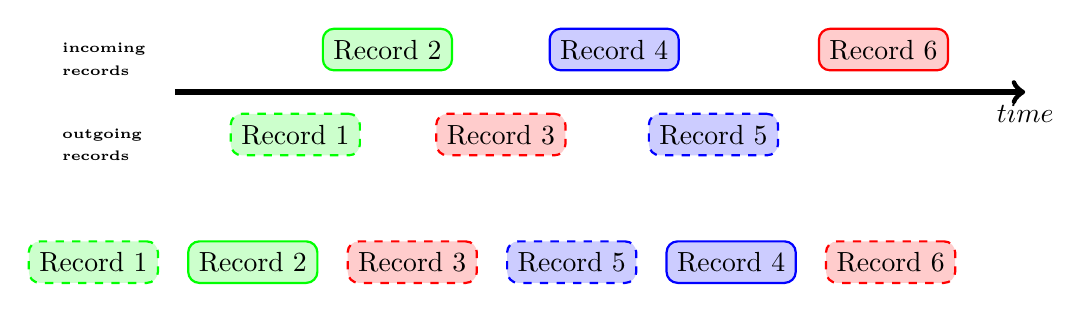
\begin{tikzpicture}[%
    scale=0.9,
    auto,
    block1/.style={
      rectangle,
      draw=blue,
      thick,
      fill=blue!20,
      text width=4em,
      align=center,
      rounded corners,
      minimum width=3em,
      minimum height=1.5em
    },
    block2/.style={
      rectangle,
      draw=green,
      thick,
      fill=green!20,
      text width=4em,
      align=center,
      rounded corners,
      minimum width=2em,
      minimum height=1.5em
    },
    block3/.style={
      rectangle,
      draw=red,
      thick,
      fill=red!20,
      text width=4em,
      align=center,
      rounded corners,
      minimum width=0.2em,
      minimum height=1.5em
    },
  ]
    \node[text width=3em] at (-2,-1.4) {\tiny\textbf{{incoming}}};
    \node[text width=3em] at (-2,-1.7) {\tiny\textbf{{records}}};
    \node[text width=3em] at (-2,-2.6) {\tiny\textbf{{outgoing}}};
    \node[text width=3em] at (-2,-2.9) {\tiny\textbf{{records}}};
    \draw [->,line width=0.7mm] (-1,-2) -- (11,-2) node[anchor=north] {$time$};
    \draw [dashed] (0.7,-2.6) node[block2] {Record 1};
    \draw (2,-1.4) node[block2] {Record 2};
    \draw [dashed] (3.6,-2.6) node[block3] {Record 3};
    \draw (5.2,-1.4) node[block1] {Record 4};
    \draw [dashed] (6.6,-2.6) node[block1] {Record 5};
    \draw (9,-1.4) node[block3] {Record 6};
    \draw [dashed] (-2.15,-4.4) node[block2] {Record 1};
    \draw (0.1,-4.4) node[block2] {Record 2};
    \draw [dashed] (2.35,-4.4) node[block3] {Record 3};
    \draw [dashed] (9.1,-4.4) node[block3] {Record 6};
    \draw [dashed] (4.6,-4.4) node[block1] {Record 5};
    \draw (6.85,-4.4) node[block1] {Record 4};
  \end{tikzpicture}
  \caption{An overview of \ac{TLS} record reordering (based on \cite{Mitseva2015})}
  \label{fig:tlsexample}
\end{figure}

In addition to \ac{TCP} data, we also extract \ac{TLS} records from the collected network traces. For that purpose, the script \texttt{raw-to-tls.py} extracts \ac{TLS} records from the original dump file using \texttt{tcpflow} and stores them in the form shown in Listing \ref{lst:tlsrawdata}. Then, similar to \texttt{parse-tcp.py}, the script \texttt{parse-tls.py} applies the \ac{IP} and timestamp matching to fetch the related connections only. In addition to the starting timestamp, \texttt{parse-tls.py} also extracts the timestamp of the \ac{TCP} packet containing the last \ac{TLS} segment as presented in Listing \ref{lst:tlsextracteddata}. This is necessary because a single \ac{TLS} record can be fragmented over multiple \ac{TCP} packets. Therefore, the data is reordered in a certain case: If a \ac{TLS} record, belonging to the communication with a given entry node, is being transferred in one direction and the transmission of a second record, belonging to the same communication, is started before the \ac{TCP} packet, containing the last fragment of the first record, is received, then the second \ac{TLS} record cannot be a response to the first record. % If a record is still being transmitted in one direction, a new record in the other direction cannot be a response to the ongoing, because it is not possible to process a record before all \ac{TCP} packets containing information regarding the same record have been received.
Figure~\ref{fig:tlsexample} illustrates an example of extracted \ac{TLS} records with their transmission time and direction. The colors of the records represent a communication with different entry nodes, i.e., in our example we consider three entry nodes. According to the duration of each transmission, we first start ordering records transferred from or to a certain entry node. Hence, we obtain the following pairs of records: 1,2 and 3,6 and 5,4. The data contained in record 4 cannot be a response of record 5 since the transmission of 4 has started before that of record 5. Afterwards, we start merging the reordered \ac{TLS} records. To do this, we compare the beginning of each \ac{TLS} record whereas we do not swap records belonging to the communication with the same entry node. In our example, we obtain the following sequence of records: 1,2,3,5,4,6. The script \texttt{parse-tls.py} does this reordering. If we enable to option \emph{legacy}, the script does not do reordering of the \ac{TLS} records, i.e., it considers the start timestamps only. 

\todo[inline]{Add newly added parsing scripts!}

\textcolor{red}{TODO: Describe the operation of check-hs-state.py, extract-main.py, parse-cells.py!}

At the end of our fetching process, the main script \texttt{fetch-and-calculate.sh} copies all collected and computed data into folder \texttt{fetches/} for further processing 

\todo[inline]{The data is copied in folder \texttt{storage/} not in \texttt{fetches/}!}

(see the organization of folder \texttt{fetches/} in Chapter \ref{chap:feature_generation}) and removes this data from folder \texttt{crawling/}. Thus, \texttt{crawling/} is ready for the next link list fetching.

\todo[inline]{Describe the option \emph{conf\_FUNCTION} located in \texttt{WFP\_config}!}

\textcolor{red}{TODO: Additionally, describe that we can either fetch traffic without processing the data or we can extract the different data layers without fetching page loads (in case that we have the collected traffic already and we want to recompute instances). Of course, the script can do both together.}

\todo[inline]{The following examples are all outdated!}
To illustrate the operation of our fetching algorithm, we consider a small example: First, we copy the generated \ac{URL} link list (see the example in Chapter 4) from folder \texttt{websiteCrawlingUrls/} into folder \texttt{crawling/}:
\vspace{-5mm}
\begin{verbatim}
# cp websiteCrawlingUrls/Urls.txt crawling/
\end{verbatim}
\vspace{-4mm}
\todo[inline]{And rename the file \texttt{Urls.txt} to \texttt{Urls}. Otherwise, you will have problems with the other scripts.}
Then, we start the main script for webpage fetching:
\vspace{-4mm}
\begin{verbatim}
# cd crawling/
# ./fetch-and-calculate.sh ../../WFP_config testRun 1 180 Urls.txt 
\end{verbatim}
\vspace{-4mm}
\todo[inline]{Show both possibilities with respect to the option \emph{conf\_FUNCTION} in \texttt{WFP\_config}!}
All measurements are directly saved into folder \texttt{fetches/} for further processing.

\section{Example files}
%\lstinputlisting[breaklines=true,language=Python,firstline=n1,lastline=n2, firstnumber=n3]{code/FILE}

\todo[inline]{Similar to the remark in Chapter~\ref{chap:list_generation}, check this example and reconstruct it in a way (if necessary) that we do not need to permanently store dummy files in the repository.}

\subsection{Input files}

The input file for fetching is the \texttt{Urls.txt} file that was created during link list creation. See Listing \ref{lst:inputUrls} for an example.

\subsection{Output files}

The following listing shows the output, consisting of the webpage \ac{URL}, timestamps and packet sizes, for the webpage \texttt{torproject.org}.
\begin{listing}[h!]
\caption{Input: \texttt{https\_\_\_www.torproject.org\_} (timestamps and sizes) \, (in folder \texttt{fetches/compiled/20150106\_121909\_test\_1\_180\_Urls\_mitseva-OptiPlex-960/output/})}
\lstinputlisting[breaklines=true,language=Python]{code/https___www.torproject.org_}
\label{lst:input1}
\end{listing}

\todo[inline]{Additional issues concerning fetching!}
\vspace{-5mm}
\begin{itemize}
  \item \textcolor{red}{Tor browser selenium (if you take a look in the old documentation, this is the previous Chickenfoot Script) which is used to manage a page load: In this script, there are different conditions used to check if a fetch is invalid (Source - the old documentation by Martin):}
  \begin{itemize}
    \item \textcolor{red}{$-1$ - Timeout (hard or soft) (needed, e.g., in case that the browser freezes)}
    \item \textcolor{red}{$-2$ - Empty page has been loaded (the \ac{URL} is about:blank)}
    \item \textcolor{red}{$-3$ - Firefox states that page has not loaded completely}
    \item \textcolor{red}{$-4$ - JavaScript Exception was thrown}
    \item \textcolor{red}{$-5$ - Waited too long for Tor streams to finish}
  \end{itemize}
\textcolor{red}{Over the years, the last condition \emph{Waited too long for Tor streams to finish} has disappeared. In the old documentation, there is no information how much one has to wait before considering a fetch as invalid. TODO: We need to revisit this!}
% check.torproject.org is removed! <-- \item \textcolor{red}{Do we still need the webpage \url{check.torproject.org}? When we load a page, we have two possibilities: $(i)$ We load foreground pages separately. This means after each foreground page (check.torproject.org + foreground page) the \ac{TBB} is restarted. $(ii)$ We load 10 background pages. This means that after 10 background pages (check.torproject.org + 10 background pages) the \ac{TBB} is restarted. In the past, the page \url{check.torproject.org} was necessary to check whether the Tor connection succeeded. Nevertheless, over the years \ac{TBB} has become much more stable. At the moment we are not using this page at all, but it is still loaded by the toolbox.}
% this is correct <-- \item \textcolor{red}{Do we correctly load a page? - After each page load, all Tor streams are closed. According to Tor specification, a circuit is closed if all streams on the corresponding circuit are closed and the lifetime of the circuit is over. Therefore, I am not sure if our foreground traces are really clean (i.e., they are loaded over a new circuit) since we first load the page \url{check.torproject.org}.}
  \item \textcolor{red}{The script \texttt{raw-to-tls.py} sometimes outputs memory error. The corresponding \ac{TLS} traces can not be extracted. Maybe problem in \texttt{tcpflow} or maybe not?}
  \item \textcolor{red}{The script \texttt{parse-tls.py} - Here, the extracting sometimes takes too long (2-3 days). Unfortunately, we did not manage to find and fix the problem.}
  \item \textcolor{red}{The scripts \texttt{check-fetches.py} and \texttt{clean-fetches.py} need improvement! They still do not clean all faulty traces.}
\end{itemize}

